\section{Tổng hợp, phản biện và thiết kế nối hai hướng nghiên
cứu}\label{tux1ed5ng-hux1ee3p-phux1ea3n-biux1ec7n-vuxe0-thiux1ebft-kux1ebf-nux1ed1i-hai-hux1b0ux1edbng-nghiuxean-cux1ee9u}

\subsection{Bảng đối chiếu mục tiêu và loại bằng
chứng}\label{bux1ea3ng-ux111ux1ed1i-chiux1ebfu-mux1ee5c-tiuxeau-vuxe0-loux1ea1i-bux1eb1ng-chux1ee9ng}

{\def\LTcaptype{none} % do not increment counter
\begin{longtable}[]{@{}
  >{\raggedright\arraybackslash}p{(\linewidth - 4\tabcolsep) * \real{0.3333}}
  >{\raggedright\arraybackslash}p{(\linewidth - 4\tabcolsep) * \real{0.3333}}
  >{\raggedright\arraybackslash}p{(\linewidth - 4\tabcolsep) * \real{0.3333}}@{}}
\toprule\noalign{}
\begin{minipage}[b]{\linewidth}\raggedright
Khía cạnh
\end{minipage} & \begin{minipage}[b]{\linewidth}\raggedright
Survey MAS/LLM
\end{minipage} & \begin{minipage}[b]{\linewidth}\raggedright
Survey RL
\end{minipage} \\
\midrule\noalign{}
\endhead
\bottomrule\noalign{}
\endlastfoot
Câu hỏi trung tâm & Ai phối hợp, bằng kênh nào, theo cơ chế nào? &
Policy học từ trải nghiệm như thế nào? \\
Đơn vị phân tích & Tác tử, kênh, tổ chức, kiến trúc & State, action,
reward, return, value \\
Vai trò dữ liệu & Ngữ cảnh, bằng chứng, message, mô hình chia sẻ &
Transition và feedback từ tương tác \\
Rủi ro & Lỗi lan truyền, đồng thuận sai, overhead & Reward lệch, mẫu
thiếu, state aliasing, bất ổn học \\
Đánh giá cần có & Quality, cost, latency, trace, ablation & Frozen
evaluation, seed, oracle, robustness \\
Liên hệ bộ mã & Shopping MAS và failure injection & E-commerce
Q-learning và DP \\
\end{longtable}
}

\subsection{Hai cấp độ thích nghi không nên
gộp}\label{hai-cux1ea5p-ux111ux1ed9-thuxedch-nghi-khuxf4ng-nuxean-gux1ed9p}

Điều phối động có thể thay graph thực hiện mà không cập nhật trọng số
một mô hình nào. Một LLM đọc feedback và sửa kế hoạch trong cùng context
có thể thay hành vi, nhưng đó chưa chứng minh có thuật toán RL tối ưu
tham số. Ngược lại, Q-learning có thể cập nhật policy trong một môi
trường có giao thức hoàn toàn cố định. ``Agent biết thích nghi'' vì thế
cần chỉ rõ thứ gì thay đổi và theo cơ chế nào.

Trong tutorial, classifier được học offline bằng nhãn và giữ cố định
trong inference. Coordinator thay trạng thái theo kết quả công cụ nhưng
không học policy phân việc. Trong assignment, Q được cập nhật trong
training rồi đóng băng để đánh giá. Ba loại thay đổi này cùng xuất hiện
trong hệ thông minh nhưng có mục tiêu và bằng chứng khác nhau.

\subsection{Thiết kế tham chiếu: trợ lý kinh doanh có tầng quyết định và
tầng kiểm
chứng}\label{thiux1ebft-kux1ebf-tham-chiux1ebfu-trux1ee3-luxfd-kinh-doanh-cuxf3-tux1ea7ng-quyux1ebft-ux111ux1ecbnh-vuxe0-tux1ea7ng-kiux1ec3m-chux1ee9ng}

Một kiến trúc nối hai hướng có thể gồm tầng nhận yêu cầu, tầng dự đoán,
tầng chọn hành động và tầng kiểm chứng. Intent classifier định tuyến
nhiệm vụ; agent dữ liệu thu thập trạng thái có version; policy learner
đề xuất mức khuyến mãi; policy validator kiểm ràng buộc; coordinator
quản lý trạng thái và dịch vụ thực thi trả xác nhận. Proposal không được
coi là một giao dịch đã thành công.

State cho learner nên chứa nhu cầu, tồn kho, lịch sử giá, ngân sách
khuyến mãi và thông tin đối thủ được phép quan sát. Action là các mức
giảm hợp lệ hoặc đề xuất giữ giá. Reward có thể dựa trên profit đã trừ
chi phí liên quan, nhưng các điều kiện pháp lý/nghiệp vụ bắt buộc phải
nằm ngoài score học. Nếu phản hồi đến muộn, cơ chế gán reward cần được
thiết kế trước khi train.

Đây là đề xuất kiến trúc, chưa được triển khai thành dịch vụ kinh doanh.
Bộ bài thực thi hai phần nhỏ có thể kiểm chứng: coordinator shopping và
learner bán hàng toy. Chúng chưa tích hợp thành hệ tự đổi giá thật; vì
thế báo cáo không đưa con số doanh thu hoặc lợi ích vận hành cho kiến
trúc mở rộng.

\subsection{Thiết kế thí nghiệm để tách lợi ích chia vai khỏi tăng tính
toán}\label{thiux1ebft-kux1ebf-thuxed-nghiux1ec7m-ux111ux1ec3-tuxe1ch-lux1ee3i-uxedch-chia-vai-khux1ecfi-tux103ng-tuxednh-touxe1n}

So sánh ít nhất bốn điều kiện: một agent với ngân sách chuẩn; một agent
với cùng tổng ngân sách như MAS; MAS đầy đủ; MAS bỏ một cơ chế phối hợp
quan trọng. Mọi điều kiện dùng cùng dữ liệu, quyền công cụ, tập tác vụ
và tiêu chí thành công. Nếu MAS được thêm nguồn dữ liệu, cần có baseline
cùng nguồn để tách ảnh hưởng dữ liệu khỏi tổ chức.

Đo success, groundedness, constraint violation, cost và latency; báo cáo
cả phân phối và các trường hợp thất bại. Với LLM, lưu prompt/model
version, nhiệt độ, số lần lấy mẫu, token và tool traces. Với RL, lưu
training steps, evaluation tapes, seed và snapshot policy. Chỉ tăng số
lần chạy mà không giữ protocol không tạo bằng chứng tái lập tốt.

Một ablation có ý nghĩa là bỏ bước inventory verification trong khi giữ
số agent khác. Nếu chất lượng giảm, kết luận hẹp là verification có ích
trong tập ca, chưa phải mọi cách chia vai đều có ích. Đây chính là cách
đọc thí nghiệm B3 của tutorial. Nhận diện đúng biến độc lập giúp tránh
gán công lao cho một nhãn kiến trúc rộng.

\subsection{Đề xuất kiểm tra độ bền nhiều
tầng}\label{ux111ux1ec1-xuux1ea5t-kiux1ec3m-tra-ux111ux1ed9-bux1ec1n-nhiux1ec1u-tux1ea7ng}

Tầng dữ liệu: thêm thiếu trường, schema sai, dữ liệu cũ và nguồn mâu
thuẫn. Tầng giao tiếp: thêm timeout, duplicate response, sai task ID và
response đến muộn. Tầng quyết định: đổi giá vốn, discount, đối thủ và
nhu cầu. Tầng triển khai: đo tải, version và cơ chế khôi phục. Mỗi thay
đổi cần giữ một tập đối chứng để xác định tác động.

Bộ mã hiện kiểm schema, freshness, timeout, forged output và shift
discount; đồng thời có self-play để minh họa đồng học. Nó chưa kiểm tải
mạng, Byzantine agent, đối thủ ngoài tập hoặc deployment thật. Một bản
báo cáo chi tiết phải ghi cả những gì đã đo và những gì chưa đo để người
đọc đặt đúng độ tin cậy.

\subsection{Những luận điểm cần tránh sau khi đọc hai
paper}\label{nhux1eefng-luux1eadn-ux111iux1ec3m-cux1ea7n-truxe1nh-sau-khi-ux111ux1ecdc-hai-paper}

Không suy ra ``nhiều agent hơn luôn đúng hơn''; sai số tương quan và chi
phí giao tiếp có thể làm kết quả kém đi. Không suy ra ``RL luôn học
policy tối ưu''; giả định Markov, tính dừng, độ bao phủ và protocol đóng
vai trò thiết yếu. Không suy ra ``accuracy cao là hệ đáng tin''; một
classifier đúng trên synthetic test vẫn nhận sai OOD. Không suy ra
``rule-based không thích ứng đầu vào''; nó có thể phản ứng theo state dù
không cập nhật từ reward.

Các kết luận tích cực vẫn rất rõ: chia vai có thể tạo hợp đồng kiểm
được; RL cung cấp cơ chế cải thiện từ feedback; model-based oracle giúp
đo khoảng cách tới chuẩn trong môi trường biết mô hình; và
logging/ablation giúp truy nguyên lỗi. Giá trị của hai paper nằm ở cách
đặt vấn đề, cộng với kiểm chứng cụ thể khi áp dụng.

\section{Bằng chứng minh họa liên hệ hai
paper}\label{bux1eb1ng-chux1ee9ng-minh-hux1ecda-liuxean-hux1ec7-hai-paper}

Các kết quả dưới thuộc bộ mã của báo cáo, không phải bảng benchmark chép
từ hai bài gốc. Tutorial kiểm kiến trúc local; assignment kiểm policy
trong mô phỏng. Phần số liệu đầy đủ nằm trong hai báo cáo chuyên biệt và
các CSV đi kèm.

{\def\LTcaptype{none} % do not increment counter
\begin{longtable}[]{@{}
  >{\raggedright\arraybackslash}p{(\linewidth - 4\tabcolsep) * \real{0.3333}}
  >{\raggedright\arraybackslash}p{(\linewidth - 4\tabcolsep) * \real{0.3333}}
  >{\raggedright\arraybackslash}p{(\linewidth - 4\tabcolsep) * \real{0.3333}}@{}}
\toprule\noalign{}
\begin{minipage}[b]{\linewidth}\raggedright
Thực nghiệm của báo cáo
\end{minipage} & \begin{minipage}[b]{\linewidth}\raggedright
Quan sát
\end{minipage} & \begin{minipage}[b]{\linewidth}\raggedright
Phạm vi kết luận
\end{minipage} \\
\midrule\noalign{}
\endhead
\bottomrule\noalign{}
\endlastfoot
MAS B0/B1 & Cùng 100\% success trên 11 ca & Chia vai chưa tăng chất
lượng trong catalog nhỏ \\
MAS B3 & 8/11 ca đúng; lỗi khi bỏ kiểm & Validation cần thiết trong tập
failure injection \\
Intent test & 108/108 đúng & Chỉ trên test tổng hợp chia nhóm \\
Intent OOD & 4/6 clarify; 2 false accept & Softmax/confidence chưa đủ
phát hiện ngoài miền \\
RL 5 seeds & 34.0997 ± 1.3678 & Baseline còn biến động và dưới policy
không giảm \\
Rule/DP & Cùng policy và khoảng 35.1295 & Best response trong mô hình
đối thủ đã chỉ định \\
\end{longtable}
}

\begin{center}
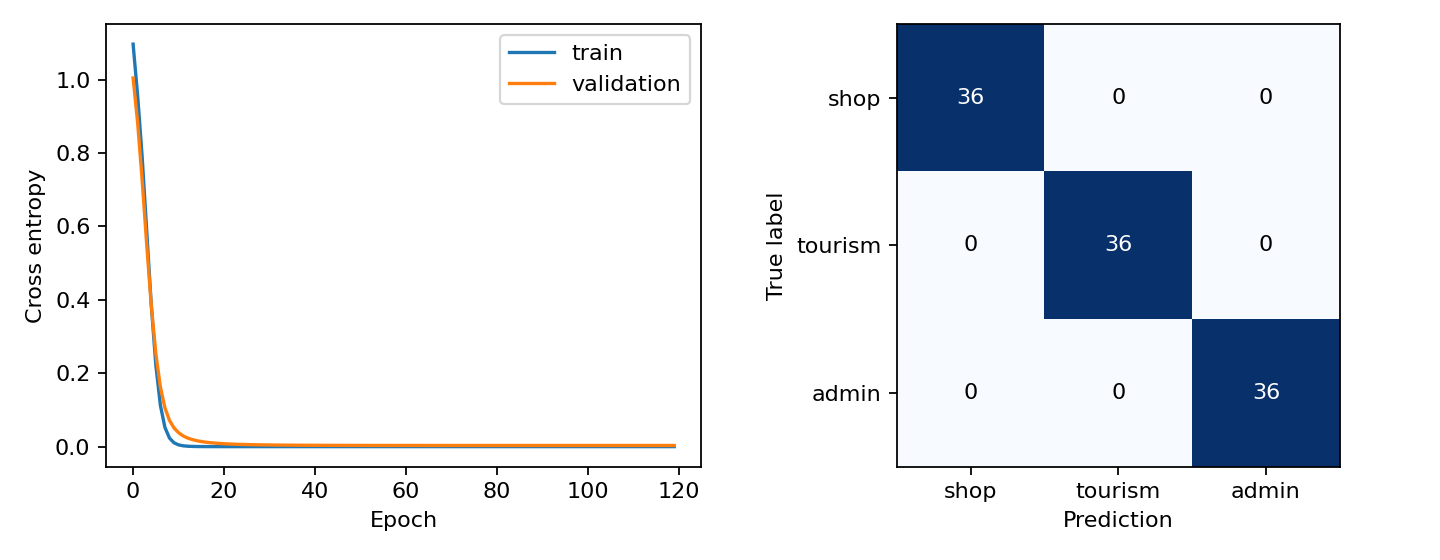
\includegraphics[width=0.98\linewidth]{results/tutorial/intent_training.png}
\captionof{figure}{Minh họa phân biệt chất lượng trong phân phối và đánh giá ngoài miền; đây là dữ liệu tự thực thi.}
\end{center}

\begin{center}
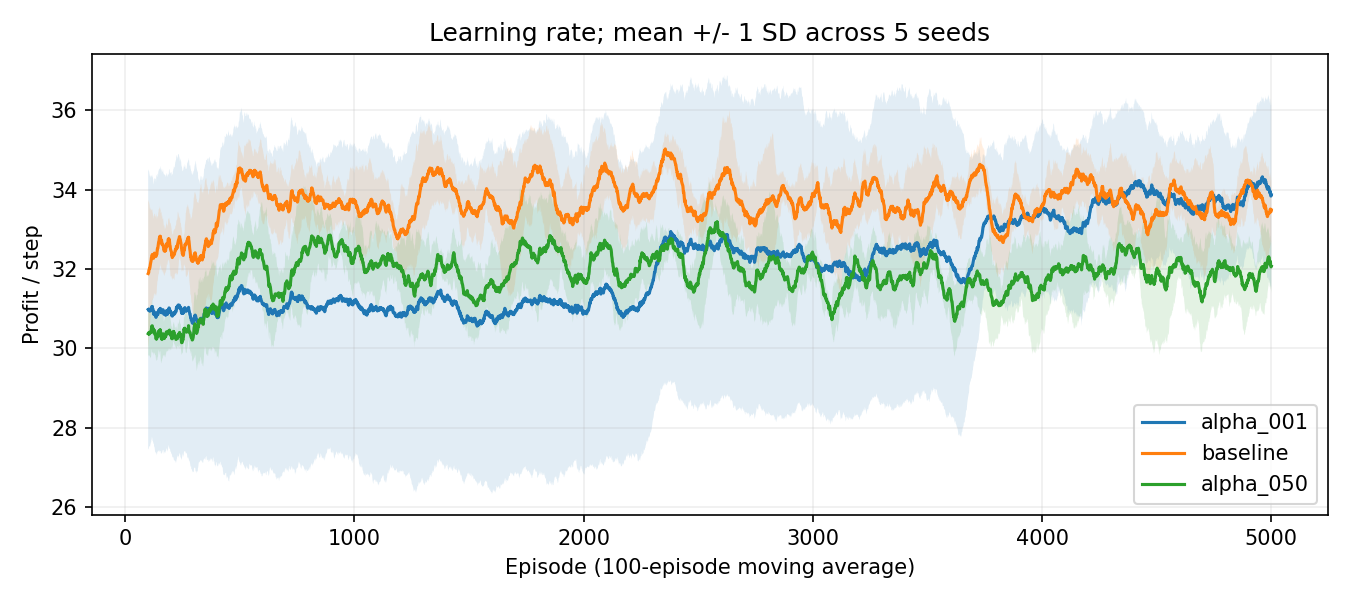
\includegraphics[width=0.98\linewidth]{results/assignment/learning_rates.png}
\captionof{figure}{Độ nhạy learning rate trong mô hình bán hàng toy; vùng tô là một SD qua năm seed.}
\end{center}

\begin{center}
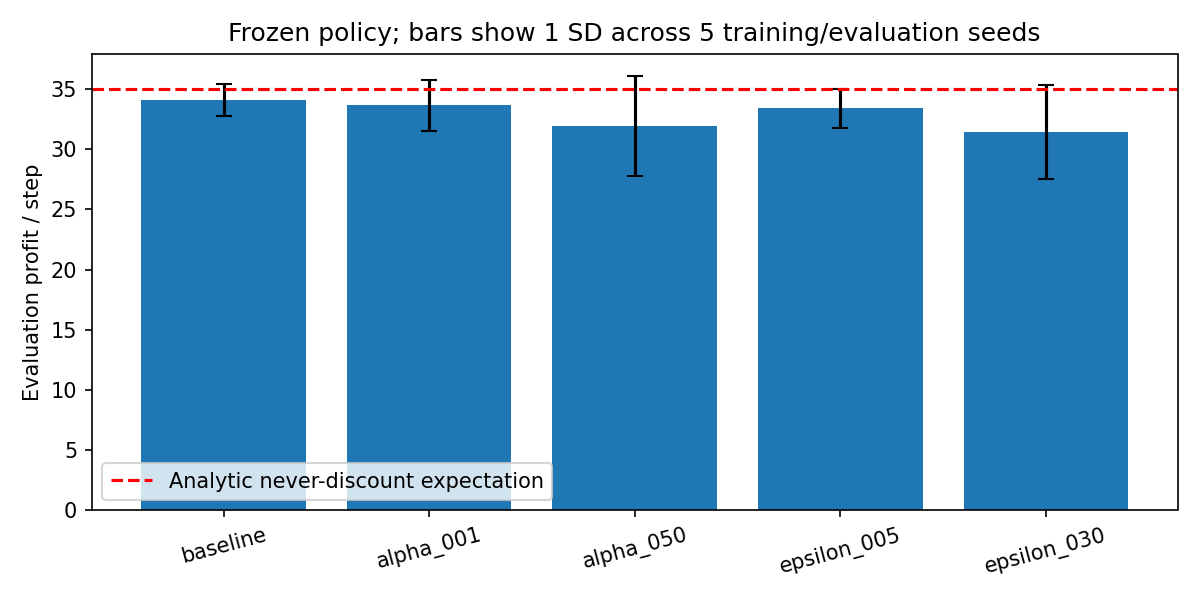
\includegraphics[width=0.98\linewidth]{results/assignment/evaluation.png}
\captionof{figure}{Đánh giá policy đóng băng và mốc analytic không giảm giá.}
\end{center}

\section{Phụ lục đọc paper: bản đồ nội dung và câu hỏi kiểm
tra}\label{phux1ee5-lux1ee5c-ux111ux1ecdc-paper-bux1ea3n-ux111ux1ed3-nux1ed9i-dung-vuxe0-cuxe2u-hux1ecfi-kiux1ec3m-tra}

\subsection{Đối chiếu Paper 1 với tài liệu
gốc}\label{ux111ux1ed1i-chiux1ebfu-paper-1-vux1edbi-tuxe0i-liux1ec7u-gux1ed1c}

{\def\LTcaptype{none} % do not increment counter
\begin{longtable}[]{@{}
  >{\raggedright\arraybackslash}p{(\linewidth - 4\tabcolsep) * \real{0.3333}}
  >{\raggedright\arraybackslash}p{(\linewidth - 4\tabcolsep) * \real{0.3333}}
  >{\raggedright\arraybackslash}p{(\linewidth - 4\tabcolsep) * \real{0.3333}}@{}}
\toprule\noalign{}
\begin{minipage}[b]{\linewidth}\raggedright
Phần tài liệu gốc
\end{minipage} & \begin{minipage}[b]{\linewidth}\raggedright
Nội dung đã phân tích
\end{minipage} & \begin{minipage}[b]{\linewidth}\raggedright
Câu hỏi khi đọc lại
\end{minipage} \\
\midrule\noalign{}
\endhead
\bottomrule\noalign{}
\endlastfoot
Section 1 & Động lực, đóng góp, vị trí survey & Tại sao cơ chế phối hợp
là trọng tâm? \\
Section 2 & MAS, LLM, collaborative AI & Mô hình khác agent ở trách
nhiệm nào? \\
Section 3 & Agent tuple, system, collaboration channel & Kênh cần mô tả
đủ những thuộc tính gì? \\
Section 4.2 & Cooperation, competition, coopetition & Mục tiêu cấp agent
và cấp hệ có khác không? \\
Section 4.3 & Rule-, role-, model-based & Đây là protocol hay decision
policy? \\
Section 4.4 & Centralized, decentralized/distributed, hierarchical &
Quyền kiểm soát khác vị trí thực thi thế nào? \\
Section 4.5 & Static/dynamic orchestration & Điểm nào thật sự thay đổi
lúc chạy? \\
Section 5 & Mạng, QA/NLG, xã hội/văn hóa & Ground truth và authority ở
đâu? \\
Section 6 & Collective intelligence, benchmark, safety & Bằng chứng nào
còn thiếu? \\
Section 7 & Kết luận taxonomy & Khung có giúp thiết kế phép thử
không? \\
\end{longtable}
}

\subsection{Đối chiếu Paper 2 với tài liệu
gốc}\label{ux111ux1ed1i-chiux1ebfu-paper-2-vux1edbi-tuxe0i-liux1ec7u-gux1ed1c}

{\def\LTcaptype{none} % do not increment counter
\begin{longtable}[]{@{}
  >{\raggedright\arraybackslash}p{(\linewidth - 4\tabcolsep) * \real{0.3333}}
  >{\raggedright\arraybackslash}p{(\linewidth - 4\tabcolsep) * \real{0.3333}}
  >{\raggedright\arraybackslash}p{(\linewidth - 4\tabcolsep) * \real{0.3333}}@{}}
\toprule\noalign{}
\begin{minipage}[b]{\linewidth}\raggedright
Phần tài liệu gốc
\end{minipage} & \begin{minipage}[b]{\linewidth}\raggedright
Nội dung đã phân tích
\end{minipage} & \begin{minipage}[b]{\linewidth}\raggedright
Câu hỏi khi đọc lại
\end{minipage} \\
\midrule\noalign{}
\endhead
\bottomrule\noalign{}
\endlastfoot
I--II & Mục tiêu, MDP/POMDP, policy, Bellman & State có đủ và quá trình
có dừng không? \\
III & Bandit, exploration, value & Feedback khác nhãn giám sát thế
nào? \\
IV-A & Dynamic programming & Biết mô hình có thể xây oracle nào? \\
IV-B & Monte Carlo & Return cần chờ đến đâu và nhiễu từ đâu? \\
IV-C & TD, SARSA, Q-learning & Target theo policy nào và có bootstrap
không? \\
IV-D/E & Actor--critic, Bayesian & Mỗi mô hình ước lượng điều gì? \\
IV-F & DQN, replay và target network & Vì sao cần ổn định khi xấp xỉ
Q? \\
V-A đến V-I & Các miền ứng dụng & Quyết định có ảnh hưởng tương lai thật
không? \\
V-J/K & Challenges, lessons learned & Reward, coverage, non-stationarity
có được kiểm? \\
VI--VII & Discussion và kết luận & Phát biểu hội tụ cần điều kiện gì? \\
\end{longtable}
}

\subsection{Câu hỏi phản biện và lời giải định
hướng}\label{cuxe2u-hux1ecfi-phux1ea3n-biux1ec7n-vuxe0-lux1eddi-giux1ea3i-ux111ux1ecbnh-hux1b0ux1edbng}

\textbf{Vì sao hai agent đồng ý vẫn có thể sai?} Vì cùng mô hình hoặc
cùng nguồn có thể gây lỗi tương quan; đa số không tạo nguồn thông tin
mới. Cần đối chiếu bằng chứng hoặc phép kiểm độc lập.

\textbf{Vì sao cùng state--action có reward khác nhau chưa chắc là
non-stationarity?} Môi trường stochastic vốn tạo reward khác qua các
mẫu. Non-stationarity nói quy luật phân phối thay đổi; cần nhiều dữ liệu
hoặc kiểm soát policy đối thủ để phân biệt.

\textbf{Vì sao tăng số seed chưa chứng minh mô hình kinh tế đúng?} Seed
chỉ thay chuỗi ngẫu nhiên trong mô hình đã giả định. Nếu conversion sai
hoặc thiếu thị phần, mọi seed đều chịu cùng sai lệch cấu trúc.

\textbf{Vì sao một agent biết mô hình có thể là baseline tốt?} Nó giúp
xác định khả năng đạt được trong mô phỏng nhỏ; chênh lệch với learner
cho thấy khoảng cách cần cải thiện. Nhưng lợi thế biết mô hình phải được
nêu để không làm so sánh thiếu công bằng về thông tin.

\textbf{Vì sao không dùng DQN cho bảng tám ô?} Không gian nhỏ không đòi
xấp xỉ bằng mạng; mạng thêm nhiễu và tuning. Chọn tabular giúp minh bạch
cập nhật và dễ đối chiếu oracle.

\textbf{Vì sao ngưỡng confidence cần validation?} Chọn trên test làm rò
rỉ thông tin về benchmark cuối. Dù chọn đúng validation, confidence vẫn
có thể cao với OOD nên cần đánh giá false acceptance riêng.

\textbf{Khi nào nên dùng MAS?} Khi có trách nhiệm, dữ liệu hoặc quyền
tách biệt và phối hợp tạo lợi ích đo được. Nếu baseline đơn đạt cùng
chất lượng với ít chi phí, lựa chọn đơn giản vẫn có cơ sở.

\textbf{Khi nào nên dùng RL?} Khi có chuỗi quyết định, feedback và điều
kiện tương tác phù hợp để học. Nếu biết mô hình nhỏ và có lời giải chính
xác, planning hoặc luật đã được kiểm chứng có thể phù hợp hơn.

\section{Kết luận chung của báo cáo
paper}\label{kux1ebft-luux1eadn-chung-cux1ee7a-buxe1o-cuxe1o-paper}

Hai paper cung cấp hai mặt bổ sung của hệ tác tử: tổ chức tương tác và
học quyết định. Một thiết kế có trách nhiệm cần cả mô hình khái niệm rõ
lẫn bằng chứng thực nghiệm phù hợp. Bản báo cáo đã trình bày nền tảng,
phân loại, công thức, thuật toán, ứng dụng, phản biện và liên hệ trực
tiếp với mã đã chạy.

Giới hạn xuyên suốt là mô phỏng toy và dữ liệu intent tổng hợp. Các con
số thực thi chứng minh quy trình và kiểm tra một số giả thuyết hẹp,
không thay thế benchmark LLM hay đánh giá vận hành thực tế. Đó là ranh
giới giúp sử dụng kiến thức từ survey một cách chính xác và có thể kiểm
tra.
